\documentclass{beamer}
\usetheme{Madrid}
%\usetheme{Goettingen}
\usefonttheme{serif}
\usefonttheme{structuresmallcapsserif}
% \usepackage[font=small,labelfont=bf]{caption}
\usepackage{xcolor}
\usepackage{rotating}
\usepackage{multirow}
\usepackage{multicol}
\usepackage{soul}

\setbeamerfont{section title}{parent=title}
\setbeamercolor{section title}{parent=titlelike}
%\defbeamertemplate*{section page}{default}[1][]
%{
%    \centering
%    \begin{beamercolorbox}[sep=8pt,center,#1]{section title}
%        \usebeamerfont{section title}\insertsection\par
%    \end{beamercolorbox}
%}

\setbeamertemplate{navigation symbols}{}
%\newcommand*{\sectionpage}{\usebeamertemplate*{section page}}

\def\Put(#1,#2)#3{\leavevmode\makebox(0,0){\put(#1,#2){#3}}}

\makeatletter
\setbeamertemplate{footline}
{
    % Commented out to remove footer line entirely
%    \leavevmode%
%    \hbox{%
%    \begin{beamercolorbox}[wd=.333333\paperwidth,ht=2.25ex,dp=1ex,center]{author in head/foot}%
%        \usebeamerfont{author in head/foot}\insertshortauthor%~~\beamer@ifempty{\insertshortinstitute}{}{(\insertshortinstitute)}
%    \end{beamercolorbox}%
%    \begin{beamercolorbox}[wd=.333333\paperwidth,ht=2.25ex,dp=1ex,center]{title in head/foot}%
%        \usebeamerfont{title in head/foot}\insertshorttitle
%    \end{beamercolorbox}%
%    \begin{beamercolorbox}[wd=.333333\paperwidth,ht=2.25ex,dp=1ex,right]{date in head/foot}%
%        \usebeamerfont{date in head/foot}\insertshortdate{}\hspace*{2em}
%        \insertframenumber{} / \inserttotalframenumber\hspace*{2ex} 
%    \end{beamercolorbox}}%
%    \vskip0pt%
}
\makeatother

\newenvironment<>{varblock}[2][\textwidth]{
    \begin{center}
        \begin{minipage}{#1}
            \setlength{\textwidth}{#1}
            \begin{actionenv}#3
                \def\insertblocktitle{#2}
                \par
                \usebeamertemplate{block begin}}
            {\par
                \usebeamertemplate{block end}
            \end{actionenv}
        \end{minipage}
    \end{center}
}

\DeclareGraphicsExtensions{.pdf,.png,.jpg}

\setbeamerfont{section title}{parent=title}
\setbeamercolor{section title}{parent=titlelike}
\defbeamertemplate*{section page}{default}[1][]
{
      \centering
      \begin{beamercolorbox}[sep=8pt,center,#1]{section title}
          \usebeamerfont{section title}\insertsection\par
      \end{beamercolorbox}
}
\newcommand*{\sectionpage}{\usebeamertemplate*{section page}}


\begin{document}
\title{Ham Radio is for Nerds}
\subtitle{\ldots like me}
\author{Josh Tolley, KG7AKX}
\frame{\titlepage}

% Ham radio used to be where aspiring hackers got started. Amateur radio is still
% a vibrant world with much to teach the interested geek. We'll talk about where
% ham radio fits in the hacker arsenal today, and cover everything you need to
% pass the FCC's licensing test and get on the air.

\section{Neat stuff radio can do}
\frame{\sectionpage}

\begin{frame}{Neat stuff radio can do}
    \begin{columns}[onlytextwidth]
        \column{0.5\textwidth}
            \begin{itemize}
                \item \only<1>{Communication between family and friends}\only<2->{\textcolor{lightgray}{Communication between family and friends}}
                \item \only<2>{Emergency preparedness}\only<1,3->{\textcolor{lightgray}{Emergency preparedness}}
                \item \only<3>{Alternative news and information sources}\only<1,2,4->{\textcolor{lightgray}{Alternative news and information sources}}
                \item \only<4>{Radio control devices}\only<1-3,5->{\textcolor{lightgray}{Radio control devices}}
                \item \only<5>{Homebrew radar}\only<1-4,6->{\textcolor{lightgray}{Homebrew radar}}
                \item \only<6>{Wireless networking}\only<1-5,7->{\textcolor{lightgray}{Wireless networking}}
                \item \only<7>{Aircraft and rocket telemetry}\only<1-6,8->{\textcolor{lightgray}{Aircraft and rocket telemetry}}
                \item \only<8>{EME / Moonbounce, satellite, space station}\only<1-7>{\textcolor{lightgray}{EME / Moonbounce, satellite, space station}}
            \end{itemize}
        \column{0.5\textwidth}
            \centering
            \only<1>{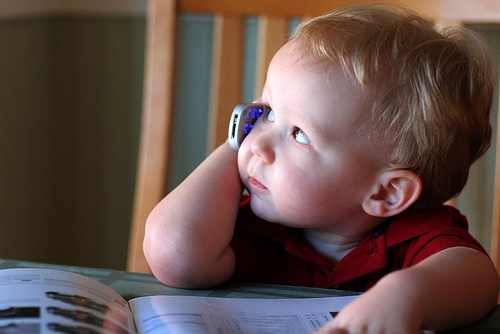
\includegraphics[width=0.9\textwidth]{img/family-friends.jpg} \\ }
            \only<2>{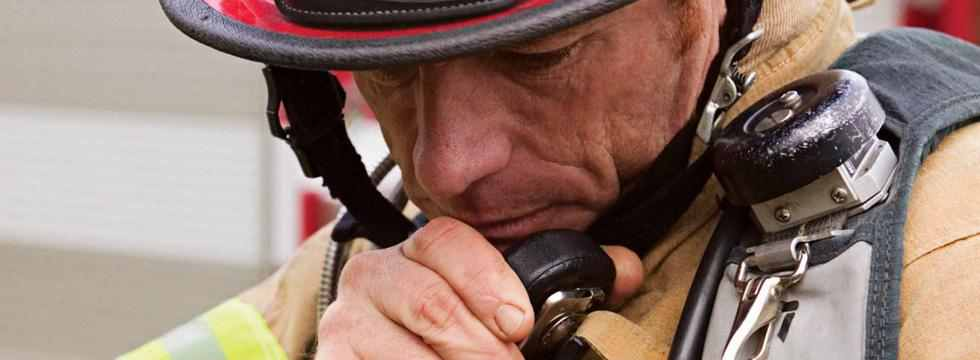
\includegraphics[width=0.9\textwidth]{img/emergency.png} \\ }
            \only<3>{
\includegraphics[width=0.9\textwidth]{img/news-info.png} \\ }
            \only<4>{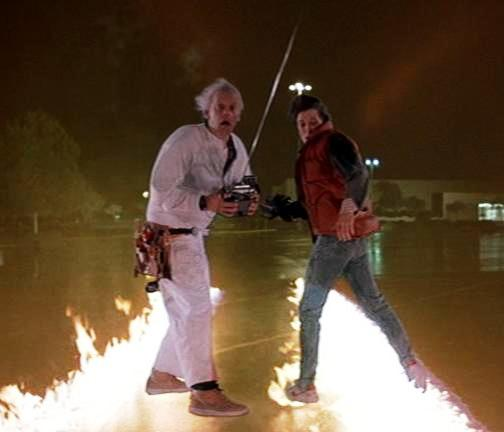
\includegraphics[width=0.9\textwidth]{img/radio-control.jpg} \\ }
            \only<5>{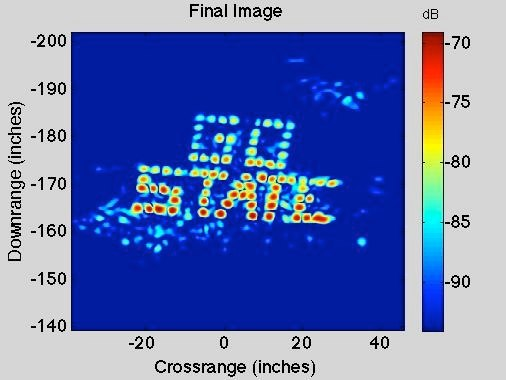
\includegraphics[width=0.9\textwidth]{img/radar.jpg} \\ }
            \only<6>{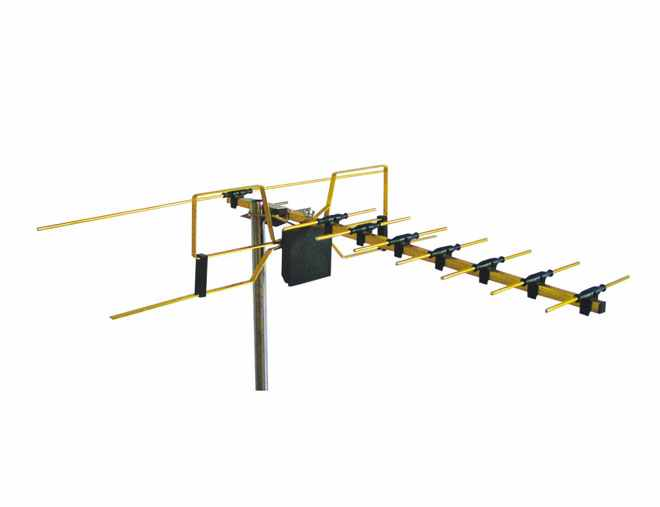
\includegraphics[width=0.9\textwidth]{img/networking.jpg} \\ }
            \only<7>{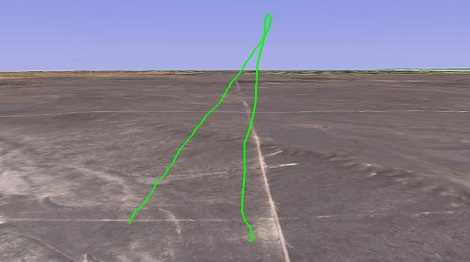
\includegraphics[width=0.9\textwidth]{img/telemetry.jpg} \\ }
            \only<8>{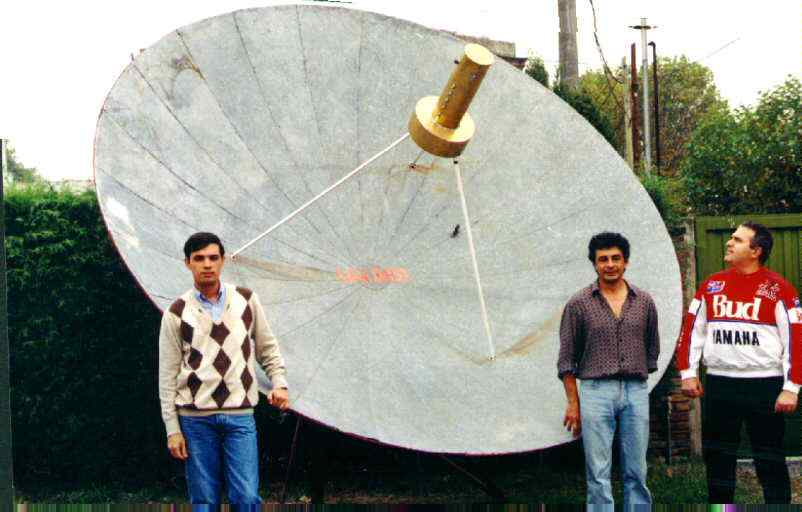
\includegraphics[width=0.9\textwidth]{img/eme.jpg} \\ }
    \end{columns}
\end{frame}

\newenvironment{proenv}{\only{\setbeamercolor{local structure}{fg=green}}}{}
\newenvironment{conenv}{\only{\setbeamercolor{local structure}{fg=red}}}{}
\newenvironment{hidenv}{\only{\setbeamercolor{local structure}{fg=white}}}{}
%\begin{frame}{test}
%    \begin{itemize}
%        \item<pro@1-> Pro
%        \pause
%        \item<con@1-> Con
%        \pause
%        \item Normal
%    \end{itemize}
%\end{frame}

\begin{frame}[t]{How radio works}
    \begin{multicols}{2}
        \begin{itemize}
            \item \only<1>{Electric field} \only<2->{\textcolor{lightgray}{Electric field}}
            \item \only<2>{Induction} \only<1,3->{\textcolor{lightgray}{Induction}}
            \item \only<3>{Carrier wave} \only<1-2,4->{\textcolor{lightgray}{Carrier wave}}
            \item \only<4>{Modulation} \only<1-3,5->{\textcolor{lightgray}{Modulation}}
            \item \only<5>{Amplification} \only<1-4,6>{\textcolor{lightgray}{Amplification}}
            \only<-5>{ \item[] }
            \only<6>{ \item Vector calculus }
        \end{itemize}
    \end{multicols}
    \centering
    \only<1>{ 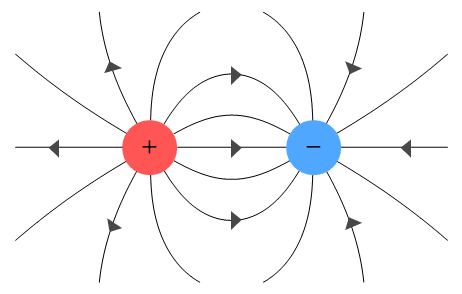
\includegraphics[height=0.6\textheight]{img/electric-field.png} \\}
    \only<2>{ 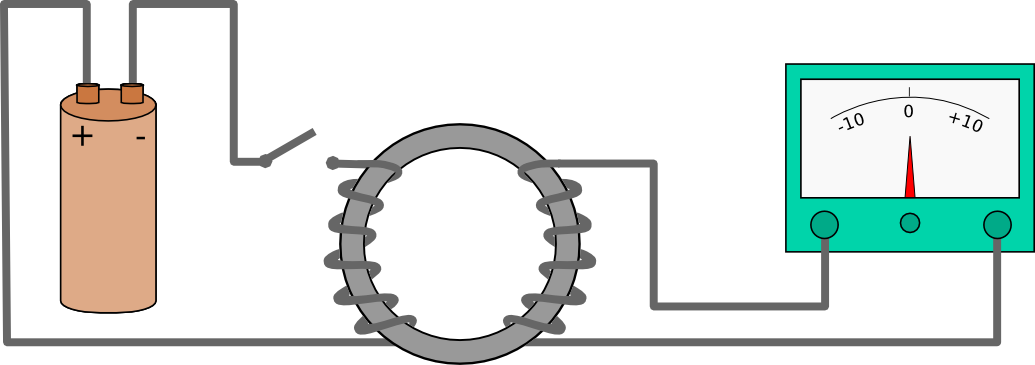
\includegraphics[height=0.6\textheight]{img/induction.png} \\}
    \only<3>{ 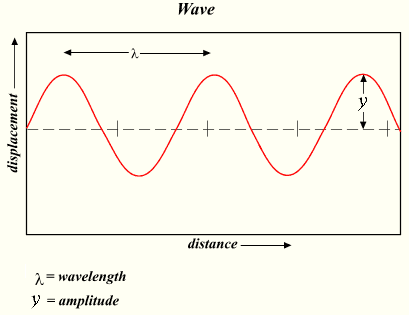
\includegraphics[height=0.6\textheight]{img/Wave.png} \\}
    \only<4>{ 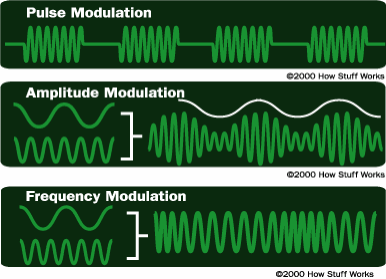
\includegraphics[height=0.6\textheight]{img/modulation.png} \\}
    \only<5>{ 
\includegraphics[height=0.6\textheight]{img/amplification.png} \\}
    \only<6>{ 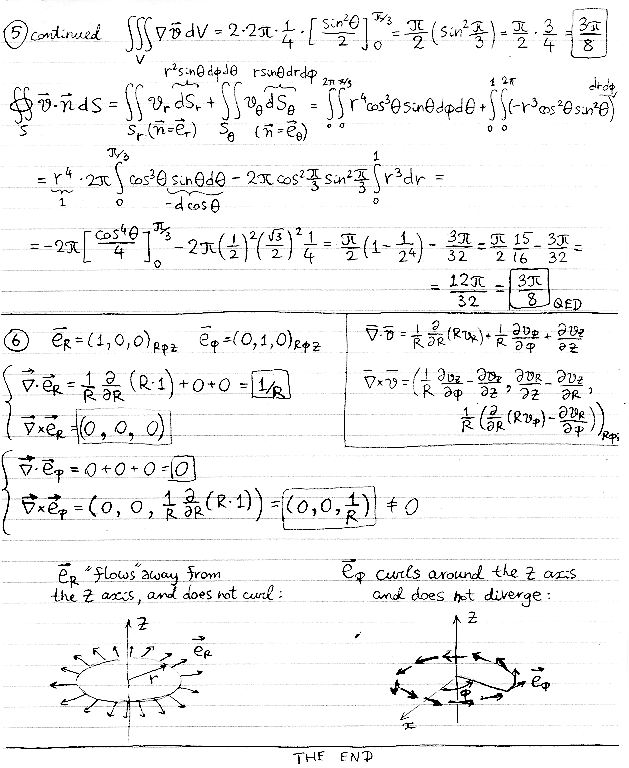
\includegraphics[height=0.6\textheight]{img/vec_cal.png} \\}
\end{frame}

\end{document}
